\documentclass[
	a4paper,
	oneside,
	BCOR = 10mm,
	DIV = 12,
	12pt,
	headings = normal,
]{scrartcl}

%%% Length calculations
\usepackage{calc}
%%%

%%% Support for color
\usepackage{xcolor}
\definecolor{lightblue}{HTML}{03A9F4}
\definecolor{red}{HTML}{F44336}
%%%

%%% Including graphics
\usepackage{graphicx}
%%%

%%% Font selection
\usepackage{fontspec}

\setromanfont{STIX Two Text}[
	SmallCapsFeatures = {LetterSpace = 8},
]

\setsansfont{IBM Plex Sans}[
	Scale = MatchUppercase,
]

\setmonofont{IBM Plex Mono}[
	Scale = MatchUppercase,
]
%%%

%%% Math typesetting
\usepackage{amsmath}

\usepackage{unicode-math}
\setmathfont{STIX Two Math}

\usepackage{IEEEtrantools}
%%%

%%% List settings
\usepackage{enumitem}
\setlist[enumerate]{
	label*      = {\arabic*.},
	leftmargin  = *,
	labelindent = \parindent,
	topsep      = 1\baselineskip,
	parsep      = 0\baselineskip,
	itemsep     = 1\baselineskip,
	noitemsep, % override itemsep
}

\setlist[itemize]{
	label*      = {—},
	leftmargin  = *,
	labelindent = \parindent,
	topsep      = 1\baselineskip,
	parsep      = 0\baselineskip,
	itemsep     = 1\baselineskip,
	noitemsep, % override itemsep
}

\setlist[description]{
	font        = {\rmfamily\upshape\bfseries},
	topsep      = 1\baselineskip,
	parsep      = 0\baselineskip,
	itemsep     = 0\baselineskip,
}

%%%

%%% Structural elements typesetting
\setkomafont{pagenumber}{\rmfamily\upshape}
\setkomafont{disposition}{\rmfamily\bfseries}

% Sectioning
\RedeclareSectionCommand[
	beforeskip = -1\baselineskip,
	afterskip  = 1\baselineskip,
	font       = {\normalsize\bfseries\scshape},
]{section}

\RedeclareSectionCommand[
	beforeskip = -1\baselineskip,
	afterskip  = 1\baselineskip,
	font       = {\normalsize\bfseries\itshape},
]{subsection}

\RedeclareSectionCommand[
	beforeskip = -1\baselineskip,
	afterskip  = 1\baselineskip,
	font       = {\normalsize\bfseries},
]{subsubsection}

\RedeclareSectionCommand[
	beforeskip = -1\baselineskip,
	afterskip  = -0.5em,
	font       = {\normalsize\mdseries\scshape\addfontfeatures{Letters = {UppercaseSmallCaps}}},
]{paragraph}
%%%

%%% Typographic enhancements
\usepackage{microtype}
%%%

%%% Language-specific settings
\usepackage{polyglossia}
\setmainlanguage{ukrainian}
\setotherlanguages{english}
%%%

%%% Captions
\usepackage{caption}
\usepackage{subcaption}

%\DeclareCaptionLabelFormat{closing}{#2)}
%\captionsetup[subtable]{labelformat = closing}

%\captionsetup[subfigure]{labelformat = closing}

\captionsetup[table]{
	aboveskip = 0\baselineskip,
	belowskip = 0\baselineskip,
}

\captionsetup[figure]{
	aboveskip = 1\baselineskip,
	belowskip = 0\baselineskip,
}

\captionsetup[subfigure]{
	labelformat = simple,
	labelformat = brace,
}
%%%

%%% Hyphenated ragged typesetting
\usepackage{ragged2e}
%%%

%%% Table typesetting
\usepackage{booktabs}
\usepackage{longtable}

\usepackage{multirow}

\usepackage{array}
\newcolumntype{v}[1]{>{\RaggedRight\arraybackslash\hspace{0pt}}p{#1}}
\newcolumntype{b}[1]{>{\Centering\arraybackslash\hspace{0pt}}p{#1}}
\newcolumntype{n}[1]{>{\RaggedLeft\arraybackslash\hspace{0pt}}p{#1}}
%%%

%%% Drawing
\usepackage{tikz}
\usepackage{tikzscale}
\usetikzlibrary{positioning}
\usetikzlibrary{arrows.meta} % Stealth arrow tips
%%%

%%% SI units typesetting
\usepackage{siunitx}
\sisetup{
	output-decimal-marker = {,},
	exponent-product      = {\cdot},
	inter-unit-product    = \ensuremath{{} \cdot {}},
	per-mode              = symbol,
}
%%%

%%% Framing code listings
\usepackage{tcolorbox}
\tcbuselibrary{breakable}
\tcbuselibrary{minted}
\tcbuselibrary{skins}

\newtcblisting[
	auto counter, 
	list inside, 
	number within = section,
]{listingpython}[3][]{%
	minted language = python,
	minted style    = bw,
	minted options  = {
		linenos,
		tabsize = 4,
		breaklines,
		% breakanywhere,
		fontsize = \footnotesize,
		autogobble
	},
	%
	% empty,
	sharp corners,
	colframe         = black,
	colback          = black!0,
	leftrule         = 0em,
	rightrule        = 0em,
	toprule          = 1pt, % orig = 0pt
	bottomrule       = 1pt, % orig = 0pt
	titlerule        = 0.5pt,
	colbacktitle     = black!0,
	coltitle         = black,
	toptitle         = 0.3em,
	bottomtitle      = 0.1em,
	borderline north = {1pt}{0pt}{black},
	borderline south = {1pt}{0pt}{black},
	before skip      = \intextsep,
	after  skip      = \intextsep,
	title            = {Лістинг \thetcbcounter: #2},
	list entry       = {\protect\numberline{\thetcbcounter}#2},
	left = 0em,
	right = 0em,
	%
	listing only,
	breakable,
	%
	label = {#3},
	%
	#1
}

\newtcbinputlisting[auto counter, list inside, number within = section]{\inputpython}[4][]{%
	minted language = python,
	minted style    = bw,
	minted options  = {
		linenos,
		tabsize = 4,
		breaklines,
		breakbytokenanywhere,
		fontsize = \footnotesize,
	},
	%
	% empty,
	sharp corners,
	colframe         = black,
	colback          = black!0,
	leftrule         = 0em,
	rightrule        = 0em,
	toprule          = 0pt, % orig = 0pt
	bottomrule       = 0pt, % orig = 0pt
	titlerule        = 0.5pt,
	colbacktitle     = black!0,
	coltitle         = black,
	toptitle         = 0.3em,
	bottomtitle      = 0.1em,
	borderline north = {1pt}{0pt}{black},
	borderline south = {1pt}{0pt}{black},
	before skip      = \intextsep,
	after  skip      = \intextsep,
	title            = {Лістинг \thetcbcounter: #3},
	list entry       = {\protect\numberline{\thetcbcounter}#3},
	left = 0em,
	right = 0em,
	%
	listing file={#2},
	listing only,
	breakable,
	%
	label = {#4},
	%
	#1
}

% Customize minted
\usepackage{minted}
\setmintedinline{
	style = bw,
	breaklines,
}

% Customize minted line numbers
\renewcommand{\theFancyVerbLine}{\ttfamily\scriptsize\arabic{FancyVerbLine}}

%%%

%%% Links and hyperreferences
\usepackage{hyperref}
\hypersetup{
	bookmarksnumbered = true,
	colorlinks      = false,
	linkbordercolor = red,
	urlbordercolor  = lightblue,
	pdfborderstyle  = {/S/U/W 1.5},
}
%%%

%%% Length adjustments
% Set baselineskip, default is 14.5 pt
\linespread{1.068966} % ~15.5 pt
\setlength{\emergencystretch}{1em}
\setlength{\parindent}{1.5em}
\newlength{\gridunitwidth}
\setlength{\gridunitwidth}{\textwidth / 12}
%%%

%%% Custom commands
\newcommand{\allcaps}[1]{{\addfontfeatures{LetterSpace = 8, Kerning = Off}#1}}
\newcommand{\filename}[1]{\texttt{#1}}
\newcommand{\progname}[1]{\texttt{#1}}
\newcommand{\modulename}[1]{\texttt{#1}}

\newcommand{\schel}[1]{\textit{#1}}
%%%

%%% Custom math commands
\newcommand{\longvar}[1]{\mathit{#1}}
%%%

\begin{document}

\begin{titlepage}
		\begin{center}
			Міністерство освіти і науки України\\
			Національний авіаційний університет\\
			Навчально-науковий інститут комп'ютерних інформаційних технологій\\
			Кафедра комп'ютеризованих систем управління

			\vspace{\fill}
				Лабораторна робота №1\\
				з~дисципліни «Діагностика та~експлуатація комп'ютера»\\
				на~тему «Діагностика блока живлення комп'ютера»\\

			\vspace{\fill}

			\begin{flushright}
				Виконав:\\
				студент \allcaps{ННІКІТ}\\
				групи СП-325\\
				Клокун В.\,Д.\\
				Перевірила:\\
				Голего Н.\,М.
			\end{flushright}

			Київ 2019
		\end{center}
	\end{titlepage}

	\section{Мета роботи}
		Ознайомлення з~методами виявлення несправностей блока живлення ком\-п'\-ют\-е\-ра. 

	\section{Хід роботи}
		\subsection{Ознайомлення з~ознаками справної роботи мережевого випрямляча і~фільтра}
			У~програмі~\textenglish{Electronics Workbench} будуємо модель мережевого випрямляча і~фільтра~(рис.~\ref{fig:ewb-rectifier}). Перевіряємо початкове положення перемикачів: \schel{K1}~— вгору, \schel{K2}~— вниз, що~відповідає роботі блока живлення від~джерела~\SI{220}{\volt}. 

			\begin{figure}[!htbp]
				\centering
				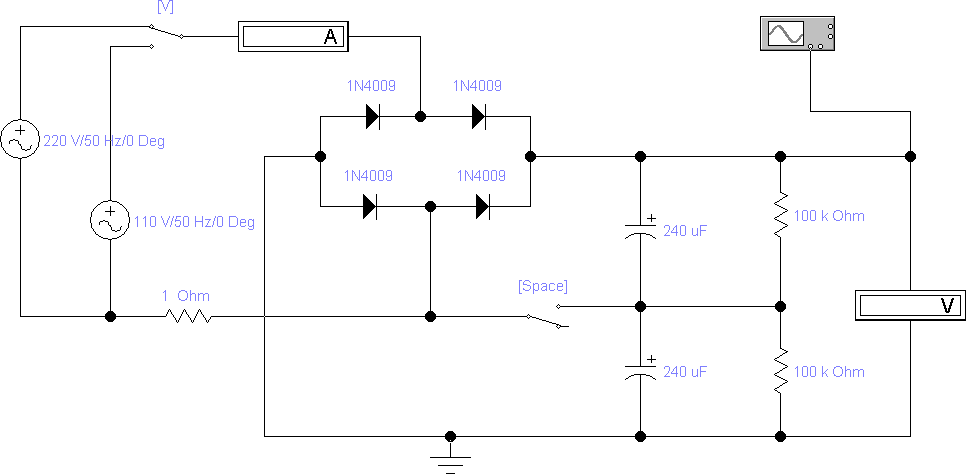
\includegraphics[height = 12\baselineskip]{./assets/y03s02-pcdiag-lab-01-p00.png}
				\caption{Електрична схема моделі мережевого випрямляча і~фільтра}
				\label{fig:ewb-rectifier}
			\end{figure}

			Ознайомлюємося з~критеріями справної роботи мережевого випрямляча при~роботі від~джерела~\SI{220}{\volt}. Для цього запускаємо моделювання необхідної схеми, спостерігаємо за~результатом та~спостерігаємо за~значеннями таких величин:
			\begin{enumerate}
				\item Вихідної напруги~$U_1$, зображеної на~вольтметрі. 
				\item Споживаного випрямлячем струму~$I_1$, зображеного на~амперметрі.
				\item Величини пульсацій випрямленої напруги~$\Delta U$. Щоб~виміряти величину пульсацій випрямленої напруги~$\Delta U$, необхідно відкрити осцилограф, встановити його у~режим змінного струму~(«\textenglish{AC}») та~виміряти амплітуду за~допомогою візирних ліній.
			\end{enumerate}
			Після стабілізації вищенаведених значень, призупиняємо моделювання, зберігаємо і~аналізуємо осцилограми~(рис.~\ref{fig:ewb-scope-01-01}). 

			\begin{figure}[!htbp]
				\centering
				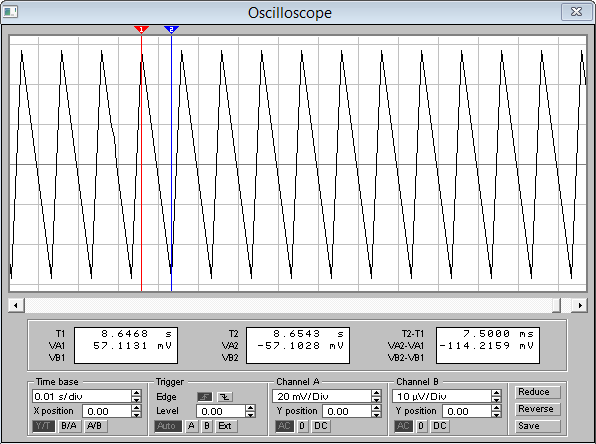
\includegraphics[height = 8\baselineskip]{./assets/y03s02-pcdiag-lab-01-p01-01b.png}
				\caption{Осцилограма вихідної напруги при~справній роботі мережевого випрямляча від~джерела живлення~\SI{220}{\volt}}
				\label{fig:ewb-scope-01-01}
			\end{figure}
			
			За даними моделювання та~отриманими осцилограмами записуємо значення величин:
			\begin{IEEEeqnarray*}{c}
				U_1 = \SI{304.5}{\volt}, \quad 
				I_1 = \SI{5.169}{\milli\ampere}, \quad
				\Delta U = \SI{114.2159}{\milli\volt}. 
			\end{IEEEeqnarray*}

			Встановлюємо перемикач~\schel{K1} у~нижню позицію, а~перемикач~\schel{K2}~— у верхню. Тепер мережевий випрямляч працює від~джерела~\SI{110}{\volt}. Запускаємо моделювання і~чекаємо стабілізації значень. Коли значення стабілізувались, призупиняємо моделювання, зберігаємо і~аналізуємо осцилограми~(рис.~\ref{fig:ewb-scope-01-02}).

			\begin{figure}[!htbp]
				\centering
				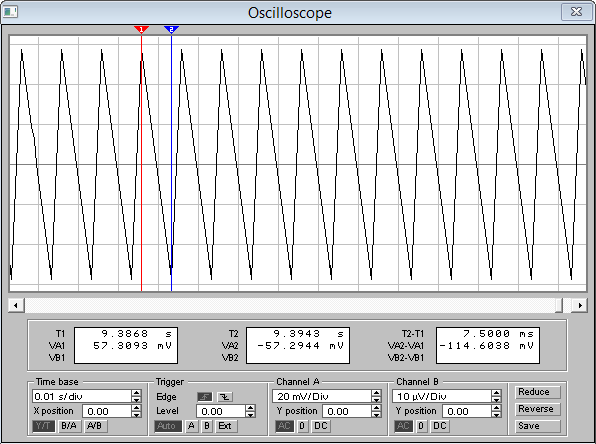
\includegraphics[height = 8\baselineskip]{./assets/y03s02-pcdiag-lab-01-p01-02b.png}
				\caption{Осцилограма вихідної напруги при~справній роботі мережевого випрямляча від~джерела живлення~\SI{110}{\volt}}
				\label{fig:ewb-scope-01-02}
			\end{figure}
			
			За даними моделювання та~отриманими осцилограмами вимірюємо необхідні значення:
			\begin{IEEEeqnarray*}{c}
				U_1 = \SI{305.5}{\volt}, \quad 
				I_1 = \SI{10.37}{\milli\ampere}, \quad
				\Delta U = \SI{114.6038}{\milli\volt}. 
			\end{IEEEeqnarray*}

			Встановлюємо перемикач~\schel{K1} у~верхню позицію. При~цьому перемикач~\schel{K2} залишаємо у~верхній. Тепер мережевий випрямляч працює від~джерела~\SI{220}{\volt} і~використовує випрямляч та~мережевий фільтр. Запускаємо моделювання і~чекаємо стабілізації значень. Коли значення стабілізувались, призупиняємо моделювання, зберігаємо і~аналізуємо осцилограми~(рис.~\ref{fig:ewb-scope-01-03}). 

			\begin{figure}[!htbp]
				\centering
				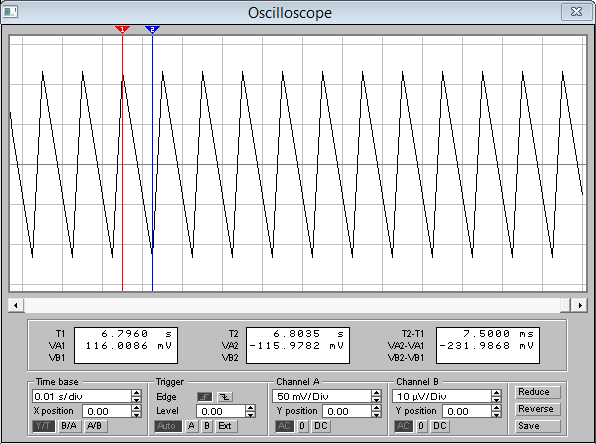
\includegraphics[height = 8\baselineskip]{./assets/y03s02-pcdiag-lab-01-p01-03b.png}
				\caption{Осцилограма вихідної напруги при~справній роботі мережевого випрямляча}
				\label{fig:ewb-scope-01-03}
			\end{figure}
			
			За даними моделювання та~отриманими осцилограмами вимірюємо необхідні значення:
			\begin{IEEEeqnarray*}{c}
				U_1 = \SI{618.5}{\volt}, \quad 
				I_1 = \SI{20.99}{\milli\ampere}, \quad
				\Delta U = \SI{231.9868}{\milli\volt}. 
			\end{IEEEeqnarray*}

		\subsection{Ознайомлення з~основними ознаками несправності мережевого випрямляча при~виході з~ладу діодів~\schel{VD1}–\schel{VD4}}
			Ознайомлюємось з~основними ознаками несправності мережевого випрямляча при~виході з~заду діодів~\schel{VD1}–\schel{VD4}. Для~цього симулюємо пробій усіх діодів, починаючи з~діода~\schel{VD1}. Щоб симулювати пробій діода, двічі натискаємо лівою клавішею миші на~бажаний діод, переходимо у~вкладку~«\textenglish{Fault}» і~обираємо тип несправності~«\textenglish{Short}». Запускаємо моделювання, спостерігаємо за результатом до~тих пір, поки стабілізуються значення, а~потім призупиняємо його. Зберігаємо і~аналізуємо осцилограми та~записуємо отримані значення вихідної напруги~$U_1$, споживаного випрямлячем струму~$I_1$ та~величини пульсацій випрямленої напруги~$\Delta U_1$. 
			
			Таким же чином симулюємо пробій кожного із~залишившихся діодів послідовно: спочатку додаємо пробій діоду~\schel{VD2}, потім~\schel{VD3} і, накінець, діода~\schel{VD4}. Повторюємо процес спостереження для~кожного експерименту, зберігаючи й~аналізуючи осцилограми~(рис.~\ref{fig:ewb-oscillograms-diod-shot}), записуємо необхідні значення та~заносимо~їх у~таблицю~(табл.~\ref{tab:diods-shot-values}). 

			\begin{figure}[!htbp]
				\centering
				\begin{subfigure}[t]{0.5\columnwidth}
					\centering
					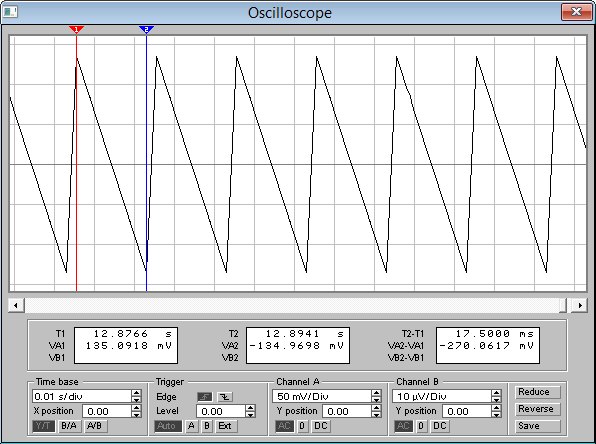
\includegraphics[height = 8\baselineskip]{./assets/y03s02-pcdiag-lab-01-p02-01b.png}
					\caption{}
					\label{subfig:ewb-scope-02-01}
				\end{subfigure}%
				\begin{subfigure}[t]{0.5\columnwidth}
					\centering
					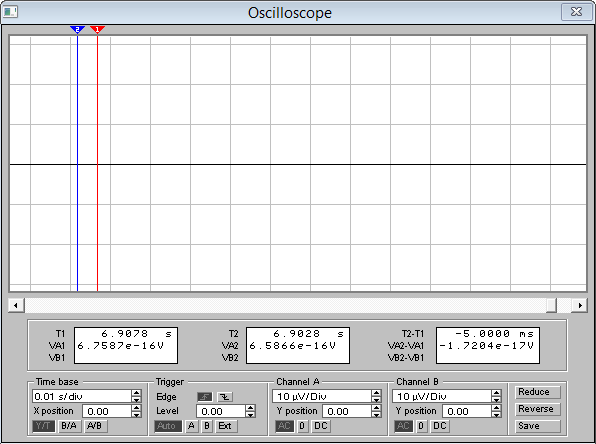
\includegraphics[height = 8\baselineskip]{./assets/y03s02-pcdiag-lab-01-p02-02b.png}
					\caption{}
					\label{subfig:ewb-scope-02-02}
				\end{subfigure}
				\begin{subfigure}[t]{0.5\columnwidth}
					\centering
					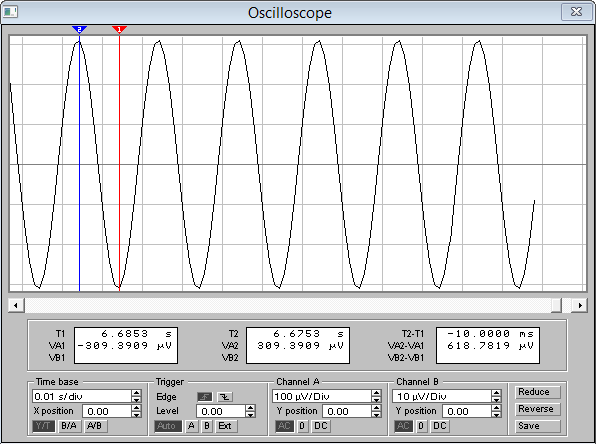
\includegraphics[height = 8\baselineskip]{./assets/y03s02-pcdiag-lab-01-p02-03b.png}
					\caption{}
					\label{subfig:ewb-scope-02-03}
				\end{subfigure}%
				\begin{subfigure}[t]{0.5\columnwidth}
					\centering
					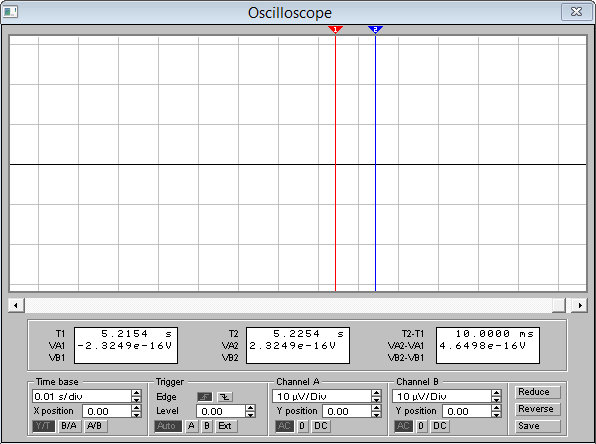
\includegraphics[height = 8\baselineskip]{./assets/y03s02-pcdiag-lab-01-p02-04b.png}
					\caption{}
					\label{subfig:ewb-scope-02-04}
				\end{subfigure}
				\caption{Осцилограми пульсацій вихідної напруги~$\Delta U_1$ при~пробої діодів: \subref{subfig:ewb-scope-02-01}~— \schel{VD1}, \subref{subfig:ewb-scope-02-02}~— \schel{VD2}, \subref{subfig:ewb-scope-02-03}~— \schel{VD3}, \subref{subfig:ewb-scope-02-04}~— \schel{VD4}}
				\label{fig:ewb-oscillograms-diod-shot}
			\end{figure}

			\begin{table}[!htbp]
				\centering
				\caption{Значення вихідної напруги~$U_1$, споживаного випрямлячем струму~$I_1$ та~величини пульсацій випрямленої напруги~$\Delta U_1$ при~пробоях діодів~\schel{VD1}–\schel{VD4}}
				\label{tab:diods-shot-values}
				\sisetup{
					table-alignment=right,
					% table-text-alignment=right,
				}
				\begin{tabular}{
						v{3.75\gridunitwidth - 2\tabcolsep}
						S[
							table-auto-round,
							table-format=1.3e+2,
							table-column-width={2.75\gridunitwidth - 2\tabcolsep},
							table-number-alignment=right,
						]
						S[
							table-auto-round,
							table-format=3.1,
							table-column-width={2.75\gridunitwidth - 2\tabcolsep},
							table-number-alignment=right,
						]
						S[
							table-auto-round,
							table-format=1.3e+2,
							table-column-width={2.75\gridunitwidth - 2\tabcolsep},
							table-number-alignment=right,
						]
				}
					\toprule
						Несправні елементи & \multicolumn{3}{r}{Виміряні значення} \\
						\cmidrule(lr){2-4}
															 & {$U_1$, \si{\volt}} & {$I_1$, \si{\ampere}} & {$\Delta U_1$, \si{\volt}}\\
					\midrule
						\schel{VD1}                                        & 3.085e+2 & 119.2 & 2.701e-1 \\
						\schel{VD1}, \schel{VD2}                           & 0.000e+0 & 219.8 & 1.7204e-17 \\
						\schel{VD1}, \schel{VD2}, \schel{VD3}              & 3.420e-6 & 219.8 & 6.188e-3 \\
						\schel{VD1}, \schel{VD2}, \schel{VD3}, \schel{VD4} & 0.000e+0 & 219.8 & 4.6498e-16 \\
					\bottomrule
				\end{tabular}
			\end{table}

			Встановлюємо справність усіх діодів. Щоб це зробити, для кожного діода відкриваємо його властивості, переходимо у~вкладку~«\textenglish{Fault}» і~встановлюємо значення~«\textenglish{None}».

		\subsection{Ознайомлення з~основними ознаками несправності конденсаторів фільтра~\schel{C1}, \schel{C2}}
			Симулюємо роботу схеми при~несправності конденсатора типу «пробій». Для~цього двічі натискаємо лівою клавішею миші на~бажаний конденсатор, переходимо у~вкладку~«\textenglish{Fault}» і~обираємо тип несправності~«\textenglish{Short}». Запускаємо моделювання та~спостерігаємо за~результатом. Записуємо значення вихідної напруги~$U_1$, споживаного випрямлячем струму~$I_1$ та~величини пульсацій випрямленої напруги~$\Delta U_1$.  

			Симулюємо роботу схеми при~несправності конденсатора типу «обрив». Для~цього двічі натискаємо лівою клавішею миші на~бажаний конденсатор, переходимо у~вкладку~«\textenglish{Fault}» і~обираємо тип несправності~«\textenglish{Open}». Запускаємо моделювання та~спостерігаємо за~результатом. Записуємо значення вихідної напруги~$U_1$, споживаного випрямлячем струму~$I_1$ та~величини пульсацій випрямленої напруги~$\Delta U_1$.  

			Повторюємо вищеописані дії для конденсатора~\schel{C2}, зберігаємо осцилограми~(рис.~\ref{fig:ewb-scope-capacitor-fault}) та~записуємо дані~(табл.~\ref{tab:capacitor-fault-values}). 

			\begin{figure}[!htbp]
				\centering
				\begin{subfigure}[t]{0.5\columnwidth}
					\centering
					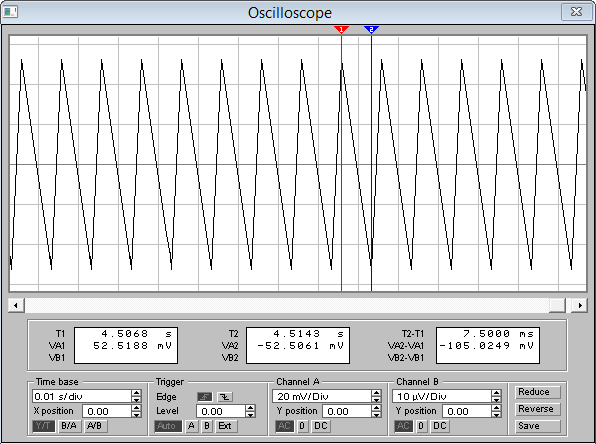
\includegraphics[height = 8\baselineskip]{./assets/y03s02-pcdiag-lab-01-p03-01b.png}
					\caption{}
					\label{subfig:ewb-scope-03-01}
				\end{subfigure}%
				\begin{subfigure}[t]{0.5\columnwidth}
					\centering
					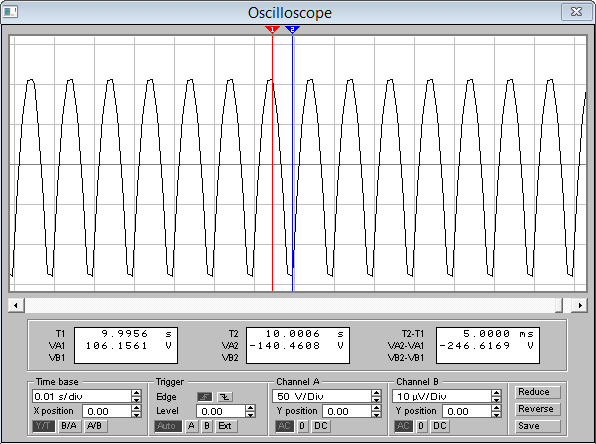
\includegraphics[height = 8\baselineskip]{./assets/y03s02-pcdiag-lab-01-p03-02b.png}
					\caption{}
					\label{subfig:ewb-scope-03-02}
				\end{subfigure}
				\begin{subfigure}[t]{0.5\columnwidth}
					\centering
					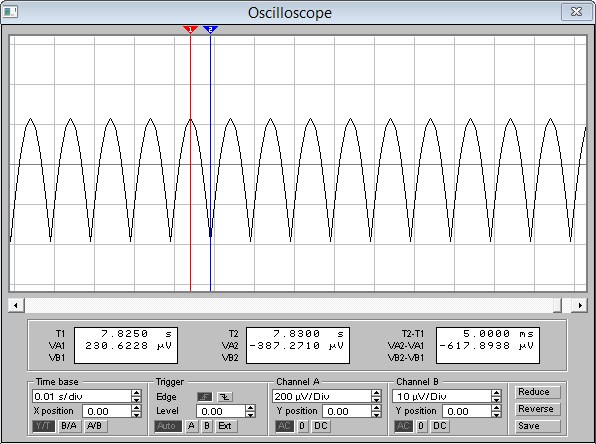
\includegraphics[height = 8\baselineskip]{./assets/y03s02-pcdiag-lab-01-p03-03b.png}
					\caption{}
					\label{subfig:ewb-scope-03-03}
				\end{subfigure}%
				\begin{subfigure}[t]{0.5\columnwidth}
					\centering
					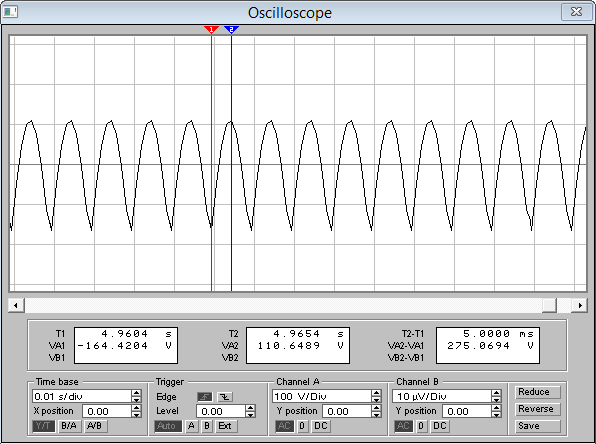
\includegraphics[height = 8\baselineskip]{./assets/y03s02-pcdiag-lab-01-p03-04b.png}
					\caption{}
					\label{subfig:ewb-scope-03-04}
				\end{subfigure}
				\caption{Осцилограми пульсацій вихідної напруги~$\Delta U_1$ при~несправностяї конденсаторів: \subref{subfig:ewb-scope-03-01}~— пробій~\schel{C1}, \subref{subfig:ewb-scope-03-02}~— обрив~\schel{C1}, \subref{subfig:ewb-scope-03-03}~— пробій~\schel{C1}, \schel{C2}, \subref{subfig:ewb-scope-02-04}~— обрив~\schel{C1}, \schel{C2}}
				\label{fig:ewb-scope-capacitor-fault}
			\end{figure}

			\begin{table}[!htbp]
				\centering
				\caption{Значення вихідної напруги~$U_1$, споживаного випрямлячем струму~$I_1$ та~величини пульсацій випрямленої напруги~$\Delta U_1$ при~несправностях конденсаторів~\schel{C1}, \schel{C2}}
				\label{tab:capacitor-fault-values}
				\sisetup{
					table-alignment=right,
					% table-text-alignment=right,
				}
				\begin{tabular}{
						v{2.25\gridunitwidth - 2\tabcolsep}
						v{1.50\gridunitwidth - 2\tabcolsep}
						S[
							table-auto-round,
							table-format=1.3e+1,
							table-column-width={2.75\gridunitwidth - 2\tabcolsep},
							table-number-alignment=right,
						]
						S[
							table-auto-round,
							table-format=1.3e+1,
							table-column-width={2.75\gridunitwidth - 2\tabcolsep},
							table-number-alignment=right,
						]
						S[
							table-auto-round,
							table-format=1.3e+1,
							table-column-width={2.75\gridunitwidth - 2\tabcolsep},
							table-number-alignment=right,
						]
				}
					\toprule
						Несправні елементи & Тип неспр. & \multicolumn{3}{r}{Виміряні значення} \\
						\cmidrule(lr){3-5}
															 & & {$U_1$, \si{\volt}} & {$I_1$, \si{\ampere}} & {$\Delta U_1$, \si{\volt}}\\
					\midrule
						\schel{C1}             & Пробій & 3.055e+2 & 9.505e-3 & 1.500249e-1 \\
						\schel{C1}             & Обрив  & 1.980e+2 & 1.947e-3 & 2.466169e+2 \\
						\schel{C1}, \schel{C2} & Пробій & 3.872e-3 & 2.180e+2 & 6.178938e-3 \\
						\schel{C1}, \schel{C2} & Обрив  & 1.973e+2 & 1.313e-3 & 2.750694e+2 \\
					\bottomrule
				\end{tabular}
			\end{table}

	\section{Висновок}
		Виконуючи дану лабораторну роботу, ми ознайомились з~методами виявлення несправностей блока живлення ком\-п'\-ю\-те\-ра.

\end{document}

